\documentclass[10pt]{article}

\usepackage{amsmath}
\usepackage{amssymb}
\usepackage[margin = 2cm]{geometry}
\usepackage{graphicx}

\usepackage{sectsty}
\sectionfont{\fontsize{12}{16}\selectfont\centering}
\subsectionfont{\fontsize{10}{14}\selectfont}

\usepackage{natbib}
\bibliographystyle{apalike}

\usepackage{hyperref}
\hypersetup{colorlinks,linkcolor={blue},citecolor={blue},urlcolor={blue}}  

\usepackage{tkz-graph}
\usetikzlibrary{arrows.meta,
	shapes.geometric}%
\tikzstyle{VertexStyle} = [shape=ellipse,
minimum width=6ex,
draw]
\tikzstyle{EdgeStyle} = [-Stealth]

\author{Gregor Steiner}
\title{Notes on Evans \& Didelez (2023)}

\begin{document}

\maketitle

This document collects my notes on \cite{evans_didelez_2023}. Consider the causal structure in Figure \ref{fig:dag}. They propose a new parameterization, termed \textbf{frugal parameterization}, which consists of three pieces: the joint distribution of the treatment and confounders $p_{ZX}(z, x)$ (the 'past'), the causal distribution of interest $p_{Y | X}^* (y|x)$, and a dependence measure between the outcome and the confounders conditional on the treatment $\phi_{YZ | X}^*$ (could be a conditional odds-ratio or a copula). In sequential treatment models, this parameterization circumvents the so-called \textbf{g-null paradox} \citep{robins_wasserman_1997}. Their main result shows that a frugal parametrization $\theta = (\theta_{ZX}, \theta_{Y|X}, \phi_{YZ | X})$ of the observational distribution induces a corresponding parameterization  $\theta^* = (\theta_{ZX}, \theta_{Y|X}^*, \phi_{YZ | X}^*)$ that is also frugal. Replacing $\theta_{ZX}$ in $\theta^*$ with $\eta_{ZX}(\theta_{ZX})$, where $\eta_{ZX}$ is a twice differentiable function with a Jacobian of constant rank, yields a parameterization of the causal joint distribution $p_{ZXY}^*$. Using this, they propose a rejection sampling algorithm to sample from $p_{ZXY}$ (implemented in the R-package \href{https://github.com/rje42/causl}{causl}). Furthermore, they show that under certain assumptions we can obtain consistent parameter estimates for the model $p_{Y | X}^*$ by maximizing the likelihood with respect to the observational data from $p_{ZXY}$. 

\begin{figure}[h] 
	\caption{Causal diagram}
	\label{fig:dag}
	\centering
	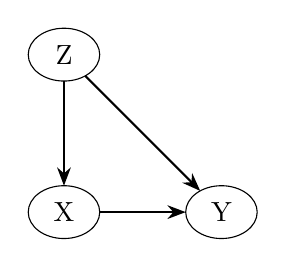
\begin{tikzpicture}[scale=2]
		\Vertex{X} \EA(X){Y} \NO(X){Z}
		\Edges(X, Y)
		\Edges(Z, Y)
		\Edges(Z, X)
	\end{tikzpicture}
\end{figure}

My understanding is that the main advantage of the frugal parameterization is that it provides a convenient characterization of the joint distribution $p_{ZXY}$, which is usually unknown or difficult to handle. Instead, we can specify a model for $p_{ZX}$ and $p_{Y | X}^*$ and choose a dependence measure of $Y$ and $Z$ conditional on $X$. Then, we can use these three to perform likelihood-based inference or simulate from the joint distribution. The joint distribution can be factorized into the frugal parameterization:

\begin{align} \label{frugal_fact}
	p_{ZXY}(z, x, y | \theta^*) &= p_{ZX}(z, x | \theta_{ZX}) p_{Y|ZX}^*(y|z, x; \theta_{Y|X}^*, \phi_{YZ | X}^*) \\
	&= p_{ZX}(z, x | \theta_{ZX}) p_{Y|X}^*(y | x; \theta_{Y|X}^*) c(y, z| x; \phi_{YZ | X}^*),
\end{align}

where $c(y, z | x; \phi_{YZ | X}^*)$ is a copula density for continuous $Y$ and $Z$ given $X$. Given observations for $(Y, X, Z)$, we can estimate $\theta^*$ by maximizing the expression above.

In their abstract, they mention that this can be used to conduct Bayesian inference, but do not discuss this in the main text. I assume this would work as follows: We can obtain a joint posterior distribution
\begin{align*}
	p(\theta^* | z, x, y) \propto p_{ZXY}(z, x, y | \theta^*) p(\theta^*),
\end{align*}
where $p(\theta^*)$ is some prior distribution. Then, we can find the posterior distribution for the parameters of the marginal model $p_{Y|X}^*$ by integrating out $\theta_{ZX}$ and $\phi_{YZ | X}^*$,
\begin{align*}
	p(\theta_{Y|X}^* | z, x, y) &= \int \int p(\theta^* | z, x, y) d\theta_{ZX} d\phi_{YZ | X}^*.
\end{align*} \\


\textbf{Comments/Questions:}
\begin{itemize}
	\item In the words of \cite{engle1983}, (\ref{frugal_fact}) implies that $[(y|z, x; \theta_{Y|X}^*, \phi_{YZ | X}^*), (z, x ;  \theta_{ZX})]$ operates a sequential cut on their joint distribution (if $(\theta_{Y|X}^*, \phi_{YZ | X}^*)$ and $\theta_{ZX}$ are variation free). Therefore, if we can find a frugal paramterization, $(x, z)$ are weakly exogenous for any function of $\theta_{Y|X}^*$. Did I get this right?
	\item What is the role of $\eta_{ZX}$?
\end{itemize}





\bibliography{references}

\end{document}
